\documentclass[12pt,pdftex,a4paper]{article}
\usepackage[ngerman]{babel}
\usepackage[utf8]{inputenc}
\usepackage{amsmath}
\usepackage{amssymb}
\usepackage{amsthm}
\usepackage{mathtools}
\usepackage{listings}
\usepackage{tikz}
\usepackage{IEEEtrantools}
\usepackage{comment}
\usepackage{xcolor}
\usepackage{graphicx}
\usepackage{ esint }

% die Verwendung von 0 bei der Spaltenangabe bei IEEEeqnarray sorgt für ein left-Alignment
%\IEEEeqnarraydefcolsep{0}{\leftmargini}\\
\newcommand{\N}{\mathbb{N}}
\newcommand{\R}{\mathbb{R}}
\newcommand{\Q}{\mathbb{Q}}
\newcommand{\Z}{\mathbb{Z}}
\newcommand{\C}{\mathbb{C}}
\newcommand{\A}{\mathcal{A}}
\newcommand{\bbI}{\mathbb{I}}
\newcommand{\bbP}{\mathbb{P}}
\newcommand{\bbF}{\mathbb{F}}
\newcommand{\ic}{\textit{i}}
\newcommand{\eu}{\text{e}}
\newcommand{\diff}{\,\mathrm{d}}
\newcommand{\h}[1]{\hat{#1}}
\newcommand{\vv}[1]{\vec{#1}}
\DeclareMathOperator{\Span}{Span}
\DeclareMathOperator{\rd}{rd}
\lstset{language=Python,basicstyle=\footnotesize}

\definecolor{darkgreen}{rgb}{0.0, 0.5, 0.0}
\definecolor{amber}{rgb}{1.0, 0.49, 0.0}
\definecolor{darkyellow}{rgb}{1.0, 0.75, 0.0}



\begin{document}
%\renewcommand{\labelenumi}{\textbf{\arabic{enumi}}}
%\renewcommand{\labelenumi}{\bfseries{\theenumi.}}
%\renewcommand{\labelenumii}{\alph{enumii})}
%\renewcommand{\labelenumii}{(\arabic{enumii})}
%\renewcommand{\labelenumi}{(\theenumi)}
\newcommand{\scale}{2.36}

\title{Numerische Simulation - Blatt 1}
\author{Mathias Feinler, Markus Schmidgall und Silvia Gramling}
\maketitle

\section*{Zu 1.6: Fragen}

\subsection*{Stabilität der Zeitschrittweite:}

\begin{table}[h]
\begin{tabular}{l|c}
  Reynoldszahl & Grenze für stabile Zeitschrittweiten  \\ \hline
  100 & 0.09-0.1 \\ 
  500 & 0.09-0.1 \\
  1 000 & 0.07-0.08 \\
  2 000 & 0.05-0.06 \\
  10 000 & 0.03-0.04\\ \hline
\end{tabular}
\caption{Obergrenzen für stabile Zeitschrittweiten in Abhängigkeit der Reynoldszahl bei 16x16 Elementen, Gittergröße von 1x1, $\alpha=1.0$ und optimalem $\omega$}
\end{table}

\newpage
\subsection*{Variation der Reynoldszahl:}

\begin{figure}[h!tb]
\centering
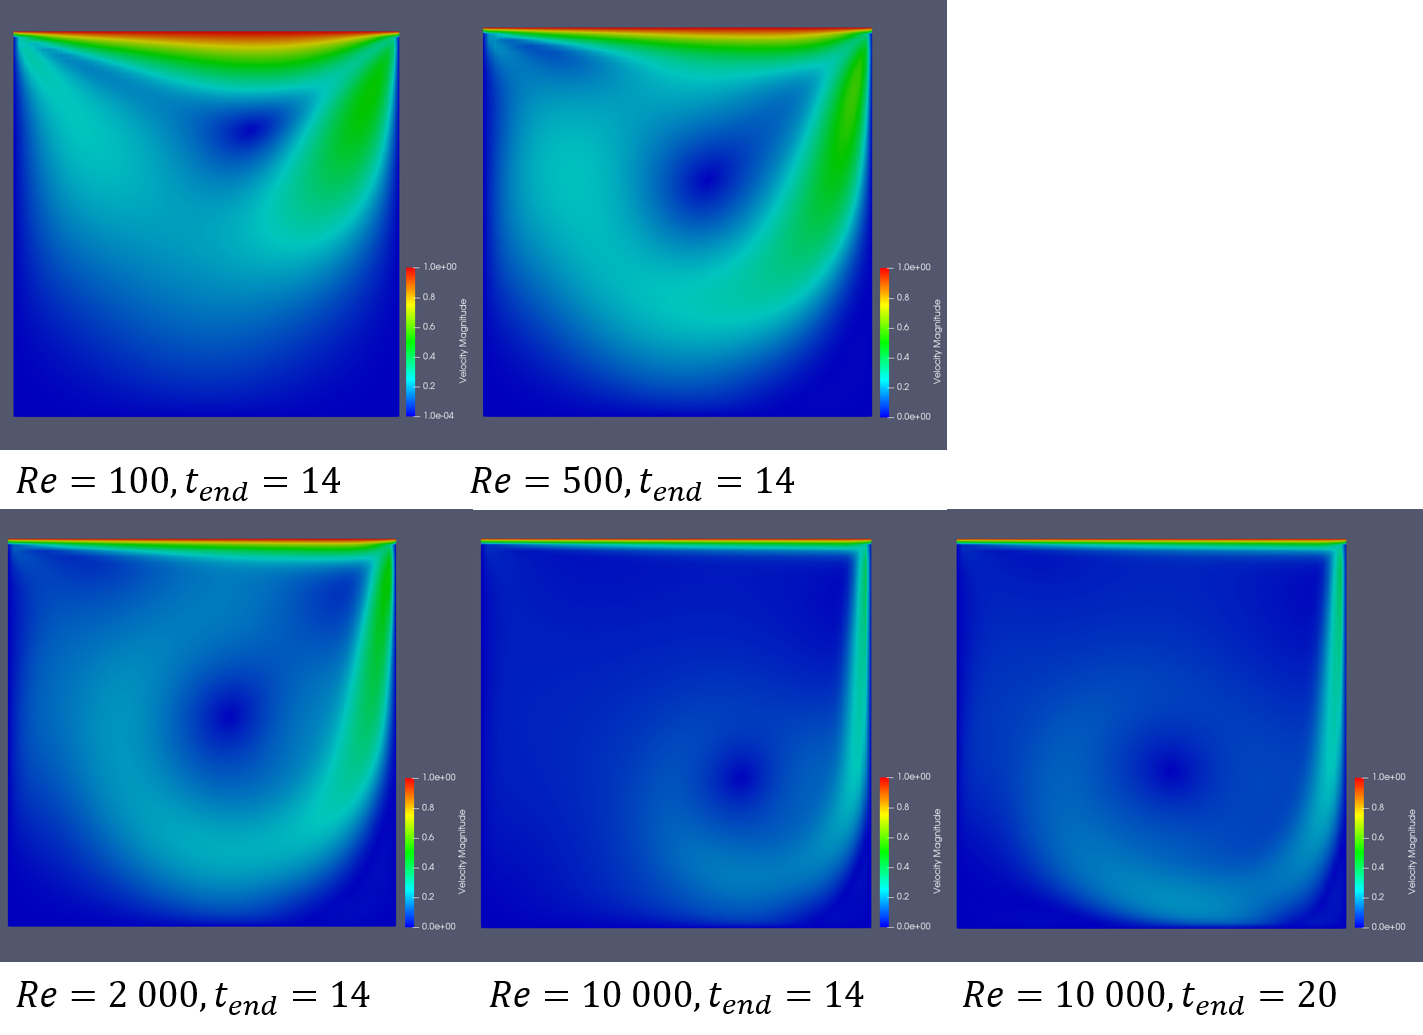
\includegraphics[width=1.0\textwidth]{pics/Reynoldszahl.png}
\caption{Geschwindigkeitsfeld für verschiedene Reynoldszahlen}
\label{fig:Re}
\end{figure}

\newpage
\subsection*{Laufzeiten:}

\begin{figure}[h!tb]
\centering
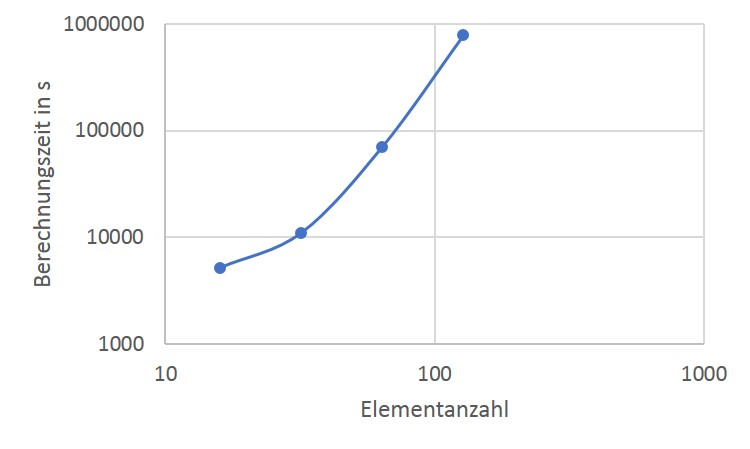
\includegraphics[width=1.0\textwidth]{pics/Berechnungszeit.jpg}
\caption{Laufzeiten in Abhängigkeit der Gitterweite bei $Re=1000$, Gittergröße von 1x1, $dt=0.01$ und $t_{end}=10$}
\label{fig:runtime}
\end{figure}

\clearpage
\section*{Anhang}

\begin{figure}[h!tb]
\centering
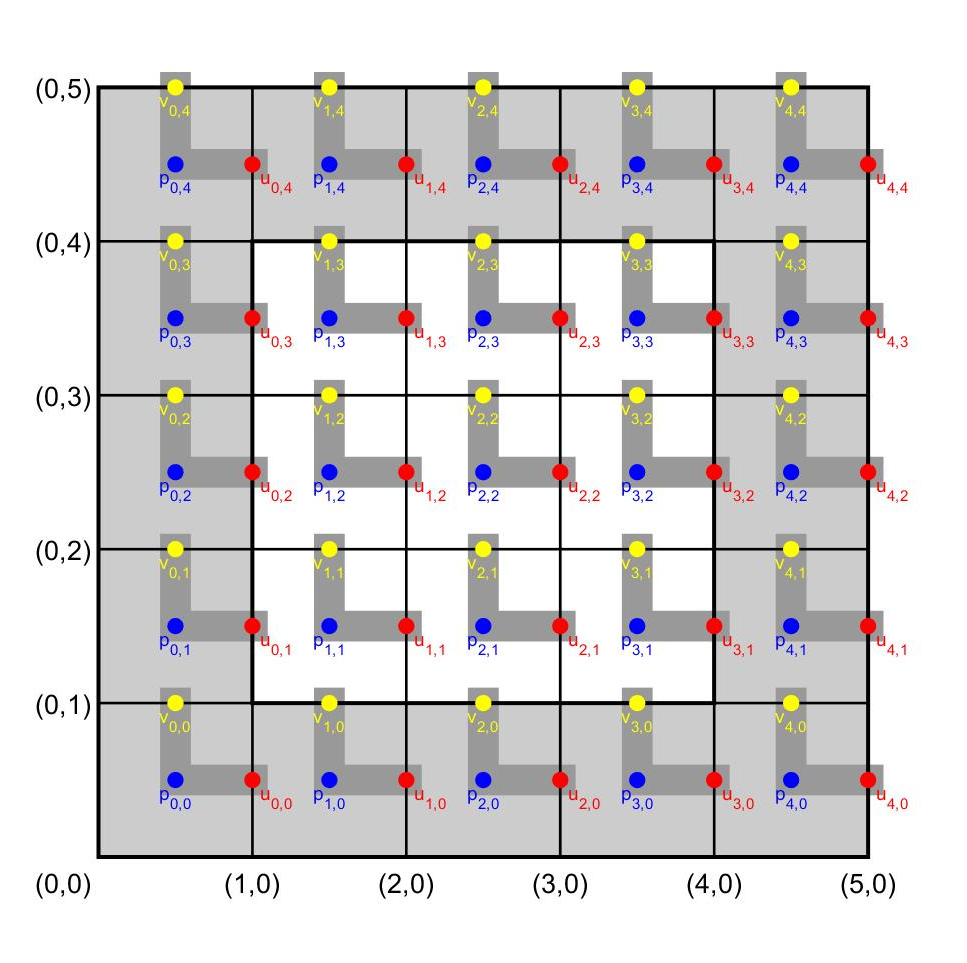
\includegraphics[width=1.0\textwidth]{pics/grid.jpg}
\caption{Staggered grid}
\label{fig:grid}
\end{figure}

\end{document}

